\documentclass[11pt]{charter}

% El títulos de la memoria, se usa en la carátula y se puede usar el cualquier lugar del documento con el comando \ttitle
\titulo{Proyecto Final} 

% Nombre del posgrado, se usa en la carátula y se puede usar el cualquier lugar del documento con el comando \degreename
%\posgrado{Carrera de Especialización en Sistemas Embebidos} 
%\posgrado{Carrera de Especialización en Internet de las Cosas} 
\posgrado{Carrera de Especialización en Inteligencia Artificial}
%\posgrado{Maestría en Sistemas Embebidos} 
%\posgrado{Maestría en Internet de las cosas}

% Tu nombre, se puede usar el cualquier lugar del documento con el comando \authorname
\autor{Ing. Alfonso Rafel} 

% FIXME:NO IMPLEMENTADO EL CODIRECTOR ni su pertenencia
\codirector{} % si queda vacio no se deberíá incluir 
\pertenenciaCoDirector{}

% Nombre del cliente, quien va a aprobar los resultados del proyecto, se puede usar con el comando \clientename y \empclientename
\cliente{Juan M. Baruffaldi}
\empresaCliente{DeepAgro}

% Nombre y pertenencia de los jurados, se pueden usar el cualquier lugar del documento con el comando \jurunoname, \jurdosname y \jurtresname y \perteunoname, \pertedosname y \pertetresname.
\juradoUno{Nombre y Apellido (1)}
\pertenenciaJurUno{pertenencia (1)} 
\juradoDos{Nombre y Apellido (2)}
\pertenenciaJurDos{pertenencia (2)}
\juradoTres{Nombre y Apellido (3)}
\pertenenciaJurTres{pertenencia (3)}
 
\fechaINICIO{18 de marzo de 2021}		%Fecha de inicio de la cursada de GdP \fechaInicioName
\fechaFINALPlanificacion{23 de abril de 2021} 	%Fecha de final de cursada de GdP
\fechaFINALTrabajo{31 de diciembre de 2021}		%Fecha de defensa pública del trabajo final


\begin{document}

\maketitle
\thispagestyle{empty}
\pagebreak


\thispagestyle{empty}
{\setlength{\parskip}{0pt}
\tableofcontents{}
}
\pagebreak

\section{Aclaración}
Para más detalle acerca del uso del código, por favor referirse al ReadMe del repositorio del proyecto en GitHub.


\section{Motivación}
\label{sec:descripcion}

El sector ganadero está en continua búsqueda de tecnologías que permitan aumentar la productividad y los márgenes de la actividad. Un área específica dentro de la ganadería es el monitoreo alimentario, que permite un control de la salud y bienestar de los animales.También constituye una herramienta para la selección de los genes más aptos.
Mediante el análisis y caracterización de los sonidos que los animales producen al comer es posible estimar la cantidad de alimento ingerido durante el pastoreo, brindando un mayor control sobre la alimentación de cada animal en un rodeo.
Los rumiantes, como las ovejas o las vacas, presentan tres tipos de movimientos
mandibulares característicos durante el pastoreo:
\begin{itemize}
	\item Masticación (o chew, del inglés): Consiste en el triturado del alimento ingerido. El animal utiliza las piezas dentarias posteriores. Se da durante la rumia y el pastoreo.
	\item Arranque (o bite, del inglés): Consiste en el corte y rasgado de la pastura. El animal utiliza las piezas dentarias anteriores. Se da únicamente en el pastoreo.
	\item Arranque-masticación (o chew-bite, del inglés): Es un solo movimiento que consiste en la combinación de los dos anteriores. Se da únicamente en el pastoreo.
 
\end{itemize}

Este trabajo consiste entonces en una solución capaz de identificar los eventos masticatorios para luego entender la actividad alimentaria de los animales.

\section{Descripción del Sistema}
\label{sec:descripcion}
La solución consiste en tres subsistemas, desarrollados en el lenguaje de programación de Python, descriptos brevemente a continuación:
\begin{itemize}
	\item Detector de eventos: este sistema se encarga de procesar el audio crudo e identificar el comienzo y el fin de los eventos. Como resultado se obtiene una serie de audios.
	\item Clasificador: este sistema clasifica los eventos previamente identificados en masticación, arranque o arranque-masticación.
	\item Actividad alimentaria: este sistema indica si el animal esta rumiando o pastoreando a partir de una ventana determinada de tiempo.
\end{itemize}

\subsection{Detector de eventos}
Para el diseño del detector de eventos utilizaremos  3 señales de audio de duración variable, con los eventos masticatorios (47, 95 y 116 respectivamente) identificados con marcas temporales. 
En primera instancia se carga un audio ejemplo y sobre el se grafican en otro color los eventos etiquetados:
\begin{figure}[H]
	\centering 
	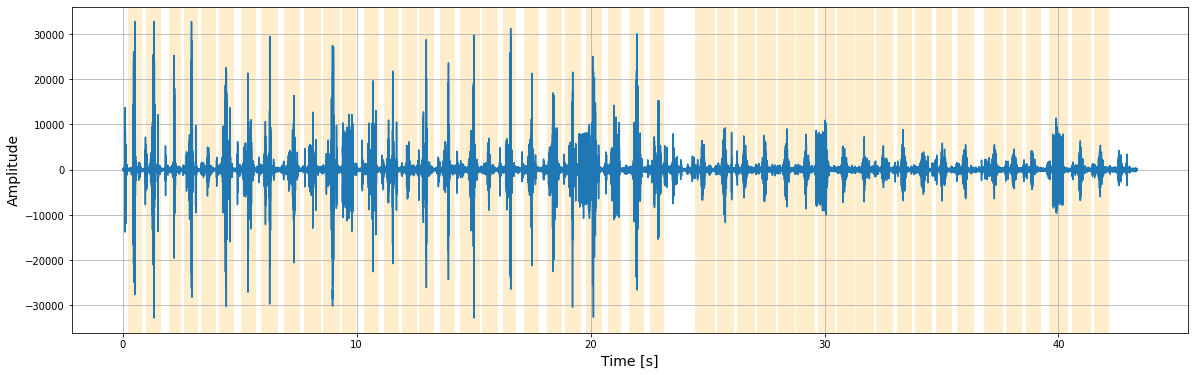
\includegraphics[width=0.9\textwidth, scale=1]{./Figuras/sample.png}
	\caption{Señal de audio muestra}
	\label{fig:sample}
\end{figure}
Del análisis frecuencial se observa un ruido de alta frecuencia a aproximadamente 4000Hz, de manera que se aplica un filtro pasabajo con una banda de paso a 2000Hz. Posteriormente, en pos de lograr una identificación más clara de las características de la señal para cada evento, se aplica un filtro pasabajos a 20Hz obteniendo como resultado lo siguiente:
\begin{figure}[H]
	\centering 
	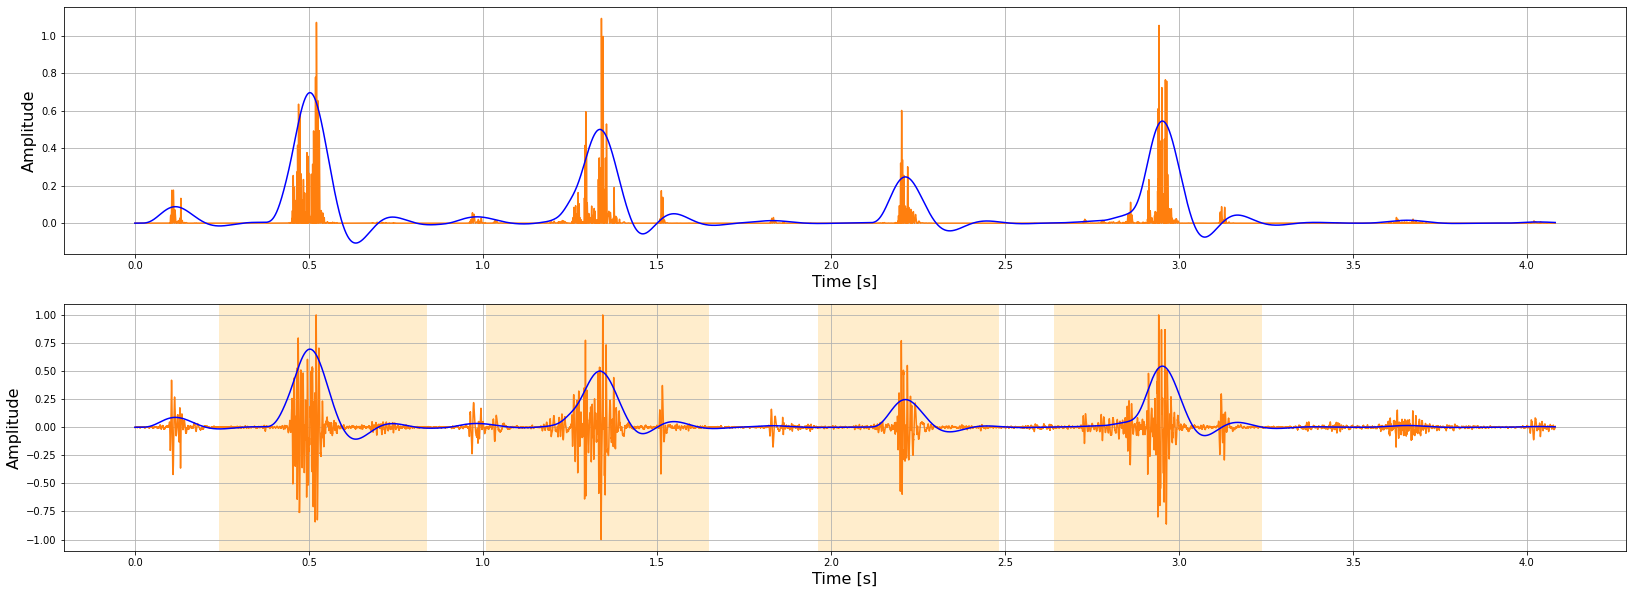
\includegraphics[width=0.9\textwidth, scale=1]{./Figuras/filter.png}
	\caption{Salida del filtro pasabajo}
	\label{fig:samplefilter}
\end{figure}
De la Figura anterior se puede apreciar la presencia de un pico de mayor amplitud y altura dentro de cada evento. De esta manera, se tienen en cuenta tres variables para la detección de estos picos:
\begin{itemize}
	\item  Magnitud: se considera una magnitud baja para poder abarcar todos los picos mayores de cada evento.
	\item Ancho: un valor mínimo de ancho de pico, dado por el promedio de los mismos, ayuda a evitar que se consideren dos picos que corresponden a eventos diferentes.
	\item Distancia: una distancia mínima entre picos, dada por el valor promedio de la duración de los eventos etiquetados, es clave para evitar separar un evento en dos.
\end{itemize}
Luego de una iteración manual considerando la traducción de tiempo en cantidad de muestras, la detección de picos arroja el siguiente resultado:
\begin{figure}[H]
	\centering 
	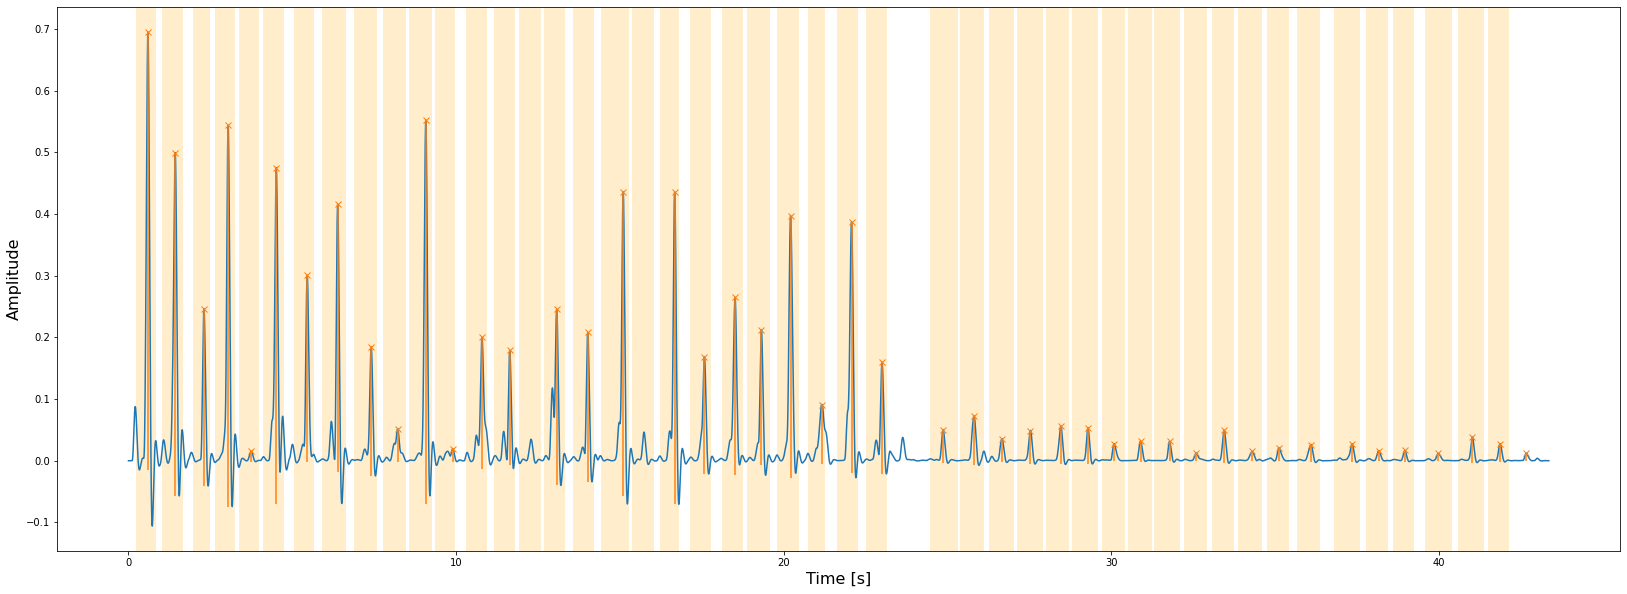
\includegraphics[width=0.9\textwidth, scale=1]{./Figuras/peaks.png}
	\caption{Detección de picos}
	\label{fig:peaks}
\end{figure}
Finalmente, para poder calcular el comienzo y el fin del evento, se considera que cada pico representa el centro del evento, y que su ancho corresponde a la media de la duración de los eventos menos la variación estándar. Tanto la media, como la variación, se calculan como el promedio de los valores de media y desviación de las 3 señales de audio. La métrica elegida para validar la precisión del sistema es IoU (Intersection over Union), la cual permite evaluar el desempeño del sistema al momento de acertar los valores exactos de comienzo y fin de los eventos. 
El valor promedio arrojado fue de 73 \%, lo cual indica que el valor fijo de ancho de evento es bueno pero aún tiene un lugar para mejoras. Respecto a la cantidad de eventos, es decir la precisión, se alcanzó en promedio un 94\%. 

\subsection{Clasificador de eventos}
Para el entrenamiento del clasificador de eventos se utilizaron un dataset con 1532 eventos individuales etiquetados dentro de las tres posibles categorías. Nos encontramos frente a un dataset sesgado, con un bajo porcentaje de arranque (16.6\%).
Como preprocesamiento se partió de la solución propuesta durante el cursado, rectificando la señal de entrada y calculando su envolvente con un filtro pasabajo. Posteriormente se procede a extraer las características que funcionarán como entradas del modelo:
\begin{itemize}
	\item Duración(duration)
	\item Cruces por zero(zero\_crossing)
	\item Amplitude(amplitud)
	\item Ratio(ratio)
	\item Desviación estándar(std)
\end{itemize}

Dado que la idea original de esta solución fue implementarla en un sistema embebido, entonces se utilizan modelos de Machine Learning relativamente simples, tales como Decision Tree, MLP y Random Forest. Para una configuración inicial de hiperparámetros se obtuvo un valor máximo de 70.4\%. Se realizó una prueba con PCA e ICA, pero se necesitaban de una cantidad de parámetros mucho mayor para lograr explicar la variabilidad de los datos.
Entendiendo la importancia que tuvieron los picos sobre la envolvente en la detección de eventos, se propusieron y pusieron a pruebas distintas variables para agregar a los modelos, tales como la potencia espectral, la energía de la señal, el valor máximo y medio de los picos, entre otras. Finalmente se agregó a la lista de variables el máximo ancho de las campanas de la envolvente, logrando así una mejora de un 2\% en el mejor modelo, alcanzando un 71.8\%.
sss
\begin{figure}[H]
	\centering 
	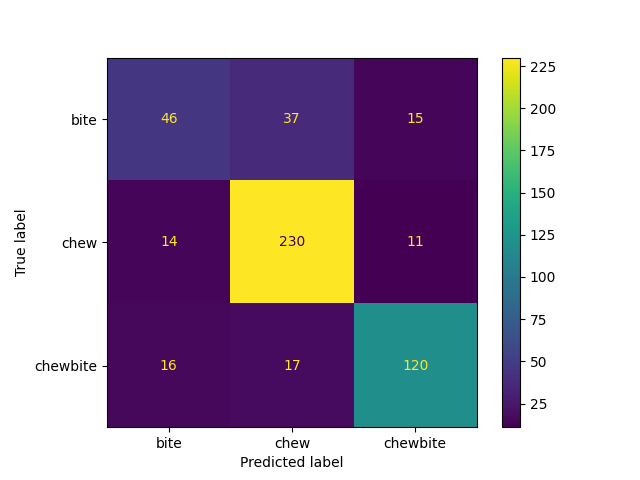
\includegraphics[width=0.5\textwidth, scale=0.5]{./Figuras/modelfirst.png}
	\caption{Matriz de Confusión}
	\label{fig:first}
\end{figure}
Finalmente se balancea el set de entrenamiento sobre el mejor modelo y además se agregan las variables mencionadas anteriormente obteniendo un balanced accuracy de 74.8\%. 
\begin{figure}[H]
	\centering 
	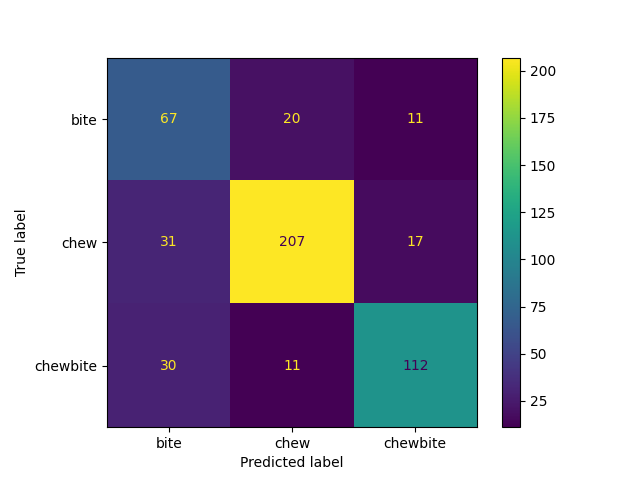
\includegraphics[width=0.5\textwidth, scale=0.5]{./Figuras/modelimbsecond.png}
	\caption{Matriz de Confusión con dataset balanceado}
	\label{fig:second}
\end{figure}
De la Figura anterior se puede observar como el balanceo genera una gran mejora en la clasificación de la clase de arranque a costa de un leve empeoramiento de las demás clases.
Finalmente se testea el conjunto modelo, es decir detector de eventos my clasificador sobre las señales de audio usadas para la clasificación. Promediando sobre los tres audios se logró un balanced accuracy de 61.7\%, lo que nos demuestra como el error del detector se propaga a la hora de la detección. 
 
\subsection{Actividad Alimentaria}
Para el entrenamiento del bloque que clasifica la actividad alimentaria se utilizó una señal de audio de aproxidamente 6 horas, en donde están etiquetadas las porciones de audio. 
En pos de generar el dataset de entrenamiento, se particionó la señal de audio en secciones de 3 minutos, sobre las cuales se aplicó la detección de eventos y posterior clasificación.
Una vez procesada cada sección se calculaban 4 parámetros y se anexaban a una tabla. Se propusieron los siguientes parámetros:

\begin{itemize}
	\item Cantidad de eventos masticatorios
	\item Porcentaje de masticación
	\item Porcentaje de arranque
	\item Porcentaje de arranque-masticación
\end{itemize}

\subsection{Próximos Pasos}
El desafío planteado revistió de una interesante dificultad, no sólo en lo que respecta al procesamiento y extracción de parámetros sobre señales de audio, sino también en el armado de un flujo de proceso completo. Es así que quedaron algunas ideas sin lograr implementarse, las cuales se incluyen como próximos pasos:
\begin{itemize}
	\item Entrenamiento conjunto: entrenamiento y validación del modelo conjunto de detección y clasicación.
	\item Uso de redes neuronales sobre las señales de audio.
	\item Uso de redes convolucionales sobre los imágenes de las curvas de las señales.
	\item División de la clase masticación en dos subclases.
	\item Uso de XAI (Explainable AI) para detectar cuales son las características faltantes de los errores de clasificación.
\end{itemize}



\end{document}
